%\documentclass{article}
\documentclass[journal,12pt,twocolumn]{IEEEtran}

% Language setting
% Replace `english' with e.g. `spanish' to change the document language
\usepackage[english]{babel}

% Set page size and margins
% Replace `letterpaper' with `a4paper' for UK/EU standard size
%%\usepackage[letterpaper,top=2cm,bottom=2cm,left=3cm,right=3cm,marginparwidth=1.75cm]{geometry}

% Useful packages
\usepackage{amsmath,amsfonts,amssymb,amsthm}
\usepackage[utf8]{inputenc}
\usepackage{enumitem}
\usepackage{multicol}
\usepackage{ragged2e}
\usepackage{amsmath}
\usepackage{amssymb}
\usepackage{graphicx}
\usepackage{listings}
%\let\vec\mathbf
%\let\myvec\bf
\usepackage{array}
\usepackage{blindtext}
%\usepackage[paperwidth=10cm]{geometry}
\usepackage{tkz-euclide}
%\usepackage{tikz}
\usetikzlibrary{
  circuits.logic,
  circuits.logic.US,
  positioning
}
\usepackage[colorlinks=true, allcolors=blue]{hyperref}
\makeatletter
\newcommand\xleftrightarrow[2][]{%
  \ext@arrow 9999{\longleftrightarrowfill@}{#1}{#2}}
\newcommand\longleftrightarrowfill@{%
  \arrowfill@\leftarrow\relbar\rightarrow}
\makeatother
\title{circle Assignment}
\author{ballepu dheeraj kumar}
\let\vec\mathbf
\begin{document}
\newcommand{\myvec}[1]{\ensuremath{\begin{pmatrix}#1\end{pmatrix}}}
\providecommand{\norm}[1]{\left\lVert#1\right\rVert}
\maketitle
\begin{tableofcontents}
\section{Problem}
\noindent  The lines 3x-4y+4=0 and 6x-8y-7=0 are tangents to the same circle.The radius of this circle is .....\\

 \section{Solution}
The distance between the two parallel lines \\
$\vec{n}^{\top}\vec{x}=\vec{C_1}$\\
$\vec{n}^{\top}\vec{x}=\vec{C_2}$\\ 
\begin{align}
\vec{D}=\frac{|\vec{C_2}-\vec{C_1}|}{\vec{\norm{n}}}
\end{align}
\vspace{2mm}
\textbf{Termux commands :}
\begin{lstlisting}
python3 circle.py
\end{lstlisting}
\begin{center}
\begin{tabular}{|c|c|c|}
\hline
\textbf{Symbol}&{Value}&{Description}\\
\hline
	\textbf{P}&$\
	\myvec{1 \\ \frac{7}{4}}$
	&Point P\\
	\hline 
\end{tabular}
\end{center}
\vspace{.25 cm}
The distance between the two parallel lines 
\begin{align}
\label{dist_3d_def_eq2}
\myvec{3 &-4}\myvec{x \\ y}=\vec{-4}
\end{align}
\begin{align}
\label{dist_3d_def_eq3}
\myvec{6 &-8}\myvec{x \\ y}=\vec{7}
\end{align}
\begin{align}
	\vec{D}=\frac{|\vec{C_2}-\vec{C_1}|}{\vec{\norm{n}}}
\end{align}
where $\vec{C_2}=3.5$,$\vec{C_1}=-4$,$\vec{\norm{n}}=5$\\
By using the above values we get $\vec D$\\
$\vec D$=1.5\\
therefore the radius of the circle is\\
$\vec R$=0.5${\vec D}$\\
Let $\vec P$ be a point on a line \eqref{dist_3d_def_eq2} \\
The equation of a line passing through point $\vec P$ and perpendicular to the line \eqref{dist_3d_def_eq2} is\\
$\vec{m}^{\top}(\vec{x}-\vec{P})=0$\\
where $\vec{m}^{\top}=\myvec{1\hspace{2mm}\frac{3}{4}}$ \\
Therefore the equation of a line passing through $\vec P$ and perpendicular to the line \eqref{dist_3d_def_eq2} is \\
\begin{align}
\label{dist_3d_def_eq5}
\myvec{16\hspace{2mm}12}\myvec{x \\ y}=\vec{37}
\end{align}
\textbf{STEP-1}\vspace{2mm}\\
 \begin{align}
       16x +12y &= 37
       \\
       6x -8y  &= 7
       \\
       \implies 
       \myvec{16 &  12
       \\
       6 & -8}\vec{X} &= \myvec{37 \\ 7}
      \end{align}
      
      The augmented matrix for the above matrix equation is 
     
     \begin{align}
       \myvec{
        16 & 12 & \vrule & 37
       \\
       6 & -8  &\vrule & 7
      }
      \\
      \xleftrightarrow[]{R_1 \leftarrow R_1/16 }
       \myvec{
        1 & 0.75 & \vrule & 2.3125
       \\
       6 & -8  &\vrule & 7
      }
      \\
      \xleftrightarrow[]{R_2 \leftarrow R_2 -6 R_1 }
       \myvec{
        1 & 0.75 & \vrule & 2.3125
       \\
       0 & -12.5  &\vrule & -6.875
      }
        \\
	     \xleftrightarrow[]{R_2 \leftarrow R_2/((-12.5) }
       \myvec{
        1 & 0.75 & \vrule & 2.3125
       \\
       0 & 1  &\vrule & 0.55
      }
        \\
	     \xleftrightarrow[]{R_1 \leftarrow R_1-(0.75)R_2 }   
	     \myvec{                   
	     1 & 0 & \vrule & 1.9  \\                         
	     0 & 1  &\vrule & 0.55
	     }
	     \\    
       \implies \vec{X} = \myvec{1.9 \\ 0.55}    
     \end{align}
So point $\vec{X}$ is a point on a line \eqref{dist_3d_def_eq3}\\
Now the midpoint of $\vec P$ and $\vec X$ gives us the centre $\vec C$= \myvec{1.45 \\ 1.15}\\
Now $\vec{\norm{P-C}}$ gives us the radius of the circle \\
$\vec{\norm{P-C}}$=0.75
\section{Construction}
 	\begin{center}
		Figure of Construction
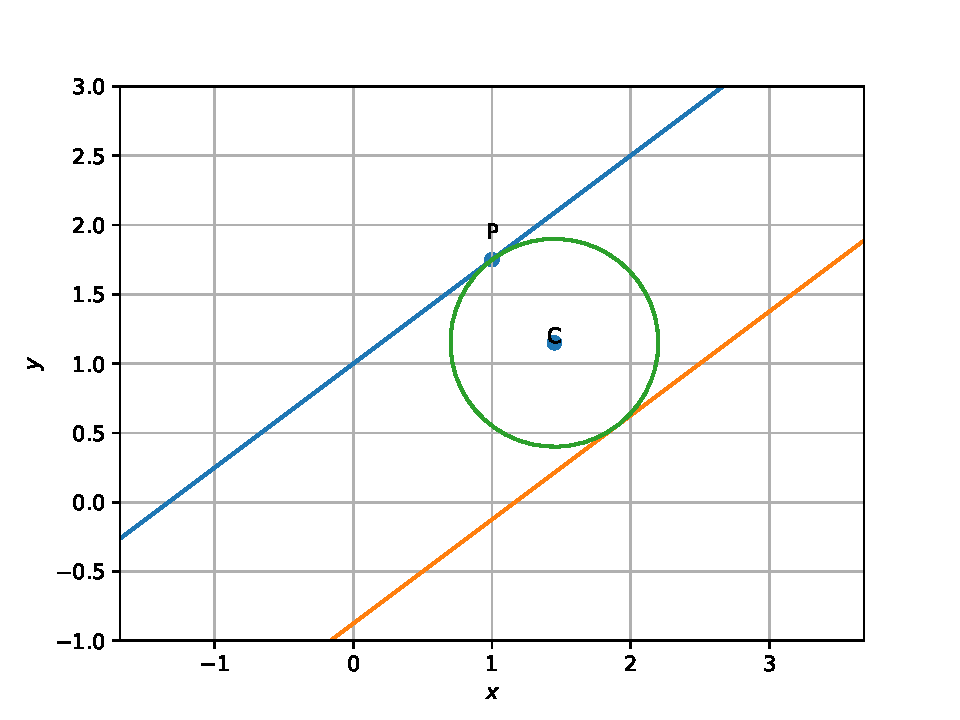
\includegraphics[scale=0.5]{/sdcard/Download/Circle/figure/fig6.pdf}
	\end{center}
  	\vspace{1mm}
The below python code realizes the above construction:	\\
\url{https://github.com/ballepu1994/matricescircle}
\bibliographystyle{ieeetr}
\end{tableofcontents}
\end{document}
